\documentclass[11pt,letterpaper]{article}

\usepackage[margin=1in]{geometry}
\usepackage[utf8]{inputenc}
\usepackage[T1]{fontenc}
\usepackage{lmodern}
\usepackage{microtype}
\usepackage{graphicx}
\usepackage{xcolor}
\usepackage{listings}
\usepackage{booktabs}
\usepackage{array}
\usepackage{longtable}
\usepackage{tabularx}
\usepackage{enumitem}
\usepackage{caption}
\usepackage{tikz}
\usetikzlibrary{positioning,arrows.meta,calc,fit,shapes.geometric,backgrounds}
\usepackage[hidelinks,colorlinks=true,linkcolor=blue,urlcolor=blue]{hyperref}

\setlength{\parskip}{0.5em}
\setlength{\parindent}{0pt}
\emergencystretch=4em
\hbadness=99999
\hfuzz=2pt

% Syntax styling for listings ------------------------------------------------
\definecolor{lstbg}{rgb}{0.97,0.97,0.97}
\definecolor{lstkw}{rgb}{0.10,0.30,0.65}
\definecolor{lstcm}{rgb}{0.40,0.40,0.40}
\definecolor{lststr}{rgb}{0.55,0.10,0.10}

\lstdefinelanguage{SystemVerilog}{
  morekeywords={module,endmodule,input,output,inout,logic,wire,reg,assign,
    always,always_ff,always_comb,always_latch,posedge,negedge,if,else,case,
    endcase,begin,end,for,while,initial,parameter,localparam,typedef,enum,
    struct,packed,unpacked,signed,unsigned,return,break,continue,default,
    int,bit,byte,shortint,longint,real,time,string,void,function,endfunction,
    task,endtask,generate,endgenerate,genvar,timescale,readmemh},
  morecomment=[l]//,
  morecomment=[s]{/*}{*/},
  morestring=[b]",
}

\lstdefinestyle{sv}{
  language=SystemVerilog,
  basicstyle=\ttfamily\footnotesize,
  keywordstyle=\color{lstkw}\bfseries,
  commentstyle=\color{lstcm}\itshape,
  stringstyle=\color{lststr},
  backgroundcolor=\color{lstbg},
  frame=single, framesep=4pt, framerule=0pt, rulecolor=\color{lstbg},
  breaklines=true, breakatwhitespace=false, columns=fullflexible, keepspaces=true,
  showstringspaces=false,
  xleftmargin=1em, xrightmargin=1em,
}

\lstdefinestyle{c}{
  language=C,
  basicstyle=\ttfamily\footnotesize,
  keywordstyle=\color{lstkw}\bfseries,
  commentstyle=\color{lstcm}\itshape,
  stringstyle=\color{lststr},
  backgroundcolor=\color{lstbg},
  frame=single, framesep=4pt, framerule=0pt, rulecolor=\color{lstbg},
  breaklines=true, breakatwhitespace=false, columns=fullflexible, keepspaces=true,
  showstringspaces=false,
  xleftmargin=1em, xrightmargin=1em,
}

\lstdefinestyle{plain}{
  basicstyle=\ttfamily\footnotesize,
  backgroundcolor=\color{lstbg},
  frame=single, framesep=4pt, framerule=0pt, rulecolor=\color{lstbg},
  breaklines=true, columns=fullflexible, keepspaces=true,
  xleftmargin=1em, xrightmargin=1em,
}

\lstset{
  style=plain,
  extendedchars=true,
  inputencoding=utf8,
  literate=%
    {→}{{$\to$}}1
    {←}{{$\leftarrow$}}1
    {↔}{{$\leftrightarrow$}}1
    {⇒}{{$\Rightarrow$}}1
    {≈}{{$\approx$}}1
    {≤}{{$\leq$}}1
    {≥}{{$\geq$}}1
    {≠}{{$\neq$}}1
    {≡}{{$\equiv$}}1
    {×}{{$\times$}}1
    {÷}{{$\div$}}1
    {±}{{$\pm$}}1
    {—}{{---}}1
    {–}{{--}}1
    {…}{{\ldots}}1
    {§}{{\S}}1
    {¶}{{\P}}1
    {∈}{{$\in$}}1
    {∉}{{$\notin$}}1
    {∞}{{$\infty$}}1
    {μ}{{$\mu$}}1
    {α}{{$\alpha$}}1
    {β}{{$\beta$}}1
    {γ}{{$\gamma$}}1
    {π}{{$\pi$}}1
    {Ω}{{$\Omega$}}1
    {°}{{$^{\circ}$}}1
    {"}{{``}}1
    {"}{{''}}1
    {'}{{`}}1
    {'}{{'}}1
}

\hypersetup{
  pdftitle={No Man's Land: A Custom SystemVerilog GPU and Game on the DE1-SoC},
  pdfauthor={Rohit Biswas, Kambinachi Obioha, Nicola Paparella},
}

% Title block ----------------------------------------------------------------
\title{\textbf{No Man's Land:}\\[0.4em]
\large A Custom SystemVerilog GPU and Game on the DE1-SoC}
\author{Rohit Biswas (rb3908) \and Kambinachi Obioha (kno2117) \and Nicola Paparella (np2953)}
\date{CSEE 4840 --- Embedded System Design, Spring 2026 \\
Instructor: Prof.\ Stephen Edwards \\
\today}

\begin{document}
\maketitle

\begin{abstract}
\noindent
No Man's Land is a top-down WWI horde-survival game implemented on the Terasic
DE1-SoC. The project partitions the system between a custom SystemVerilog GPU
peripheral (\texttt{nml\_gpu}) running in the Cyclone V FPGA fabric and a C game
on the ARM Cortex-A9 hard processor. The GPU drives a 640$\times$480 @ 60\,Hz
VGA output with tile-mapped background, 32 hardware sprites with per-scanline
priority sorting, a 256-entry palette, and an on-chip HUD overlay. The HPS
writes the sprite table, palette, tile map, and player-state registers through
a 16\,KB Avalon-MM lightweight slave and signals a tear-free buffer swap at
VBLANK. Two build flows exist: a fabric-only smoke test
(\texttt{hw/quartus}) that confirms the rendering pipeline by initialising the
memories from \texttt{\$readmemh} hex files, and an HPS-integrated Platform
Designer system (\texttt{nml\_gpu\_hw/}) that mounts the peripheral on the
lightweight bridge and exposes it to a Linux userspace driver via
\texttt{/dev/mem}. The smoke-test bitstream is verified on hardware. The
HPS-integrated build boots Linux, exposes the peripheral on the lightweight
bridge, runs the C game loop at 60\,Hz, drives the VGA monitor, and reads SNES
controller input through evdev. This report covers the architecture, register
map, build flow, and verified results.
\end{abstract}

\newpage
\tableofcontents
\newpage

% ===========================================================================
\section{Introduction}

The course's final-project remit is to design and integrate a custom
SystemVerilog peripheral that drives a VGA display and to write a C
application that uses the peripheral to do something interesting. We chose a
WWI-themed horde-survival game on the principle that it stresses both sides:
the FPGA must composite many sprites per scanline at pixel rate, and the CPU
must run wave logic, enemy AI, projectile physics, collision checks, an
auto-attack system, and a HUD-driven UI within a 16.67\,ms frame budget.

The player controls a soldier in a trench at the bottom of the screen. Waves
of enemies spawn at the top and march down. The player fires bullets in four
directions, picks up ammo drops, and at the end of each wave selects an
auto-attack upgrade (mortar, mustard gas, or artillery). The goal is to
survive as many waves as possible.

Input is a SNES-style USB gamepad (DragonRise generic, VID 0079:0011) read
through Linux evdev. A keyboard fallback was explicitly disallowed by the
instructor; we kept a deterministic stub input (\texttt{input\_fake.c}) for
off-line development and demos when the controller is unavailable.

The deliverables and supporting documents are:

\begin{itemize}[leftmargin=*,nosep]
  \item \texttt{DESIGN.md} --- the original design document with system block diagram, register map, and game design.
  \item \texttt{SETUP.md} --- bring-up instructions: host sanity check, JTAG smoke test, and HPS integration on the SD-card image.
  \item This report and the companion internal deep-dive (\texttt{docs/internal\_deep\_dive.md}).
\end{itemize}

% ===========================================================================
\section{System Architecture}

The system is partitioned along the obvious line: anything that runs at pixel
rate is in hardware; everything else is in software. The block diagram is
shown in Figure~\ref{fig:sysblock}.

\begin{figure}[h]
\centering
\resizebox{\textwidth}{!}{%
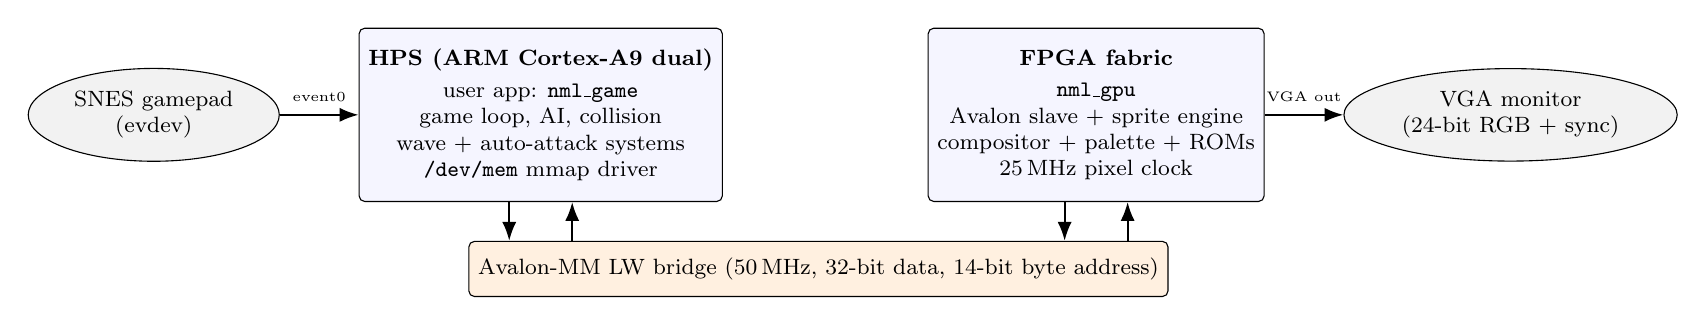
\begin{tikzpicture}[
  font=\footnotesize,
  block/.style={draw, rectangle, rounded corners=2pt, minimum width=4.0cm, minimum height=2.2cm, align=center, fill=blue!4},
  io/.style={draw, ellipse, minimum width=2.4cm, minimum height=1.0cm, align=center, fill=gray!10},
  bus/.style={draw, rectangle, minimum width=5.4cm, minimum height=0.7cm, align=center, fill=orange!12, rounded corners=2pt},
  arr/.style={-{Latex[length=2.4mm]}, thick},
  >={Latex[length=2.4mm]},
]
  \node[block] (hps) {\textbf{HPS (ARM Cortex-A9 dual)} \\[2pt]
    user app: \texttt{nml\_game} \\
    game loop, AI, collision \\
    wave + auto-attack systems \\
    \texttt{/dev/mem} mmap driver};
  \node[block, right=2.6cm of hps] (fpga) {\textbf{FPGA fabric} \\[2pt]
    \texttt{nml\_gpu} \\
    Avalon slave + sprite engine \\
    compositor + palette + ROMs \\
    25\,MHz pixel clock};
  \node[io, left=1.0cm of hps] (pad) {SNES gamepad \\ (evdev)};
  \node[io, right=1.0cm of fpga] (vga) {VGA monitor \\ (24-bit RGB + sync)};
  \node[bus, below=1.6cm of $(hps)!0.5!(fpga)$] (bus) {Avalon-MM LW bridge (50\,MHz, 32-bit data, 14-bit byte address)};

  % Bidirectional bus traffic --- two arrows side-by-side under each block
  \draw[arr] ([xshift=-4mm]hps.south) -- ([xshift=-4mm]hps.south |- bus.north);
  \draw[arr] ([xshift=4mm]hps.south |- bus.north) -- ([xshift=4mm]hps.south);
  \draw[arr] ([xshift=-4mm]fpga.south) -- ([xshift=-4mm]fpga.south |- bus.north);
  \draw[arr] ([xshift=4mm]fpga.south |- bus.north) -- ([xshift=4mm]fpga.south);

  % I/O peripherals on the sides
  \draw[arr] (pad.east) -- (hps.west) node[midway, above=1pt] {\tiny event0};
  \draw[arr] (fpga.east) -- (vga.west) node[midway, above=1pt] {\tiny VGA out};
\end{tikzpicture}}
\caption{System block diagram. HPS runs the C game; FPGA fabric runs the GPU peripheral; the lightweight bridge carries register writes and reads between them.}
\label{fig:sysblock}
\end{figure}

The HPS reads input from the USB gamepad, ticks the game state at 60\,Hz,
writes the resulting sprite table, palette, and tile map into FPGA memory
through the Avalon-MM lightweight slave, and signals a frame swap by writing
the \texttt{CTRL.SWAP} bit. The FPGA latches the new state at the next VSYNC
and continues to drive the monitor without ever stalling. A 50\,MHz Avalon
clock and a 25\,MHz pixel clock are the only two clock domains in the design;
both derive from the board's 50\,MHz oscillator.

Frame budget at 60\,Hz is 16.67\,ms. Per VGA frame at 640$\times$480 there are
$800 \times 525 = 420{,}000$ pixel cycles at 25\,MHz (16.8\,ms wall-clock), of
which $640 \times 480 = 307{,}200$ are visible. The 96-pixel horizontal
blanking and multi-line vertical blanking give the sprite engine the time it
needs to prepare each scanline.

% ===========================================================================
\section{Hardware Design}

The hardware lives in \texttt{hw/} and consists of seven SystemVerilog modules
plus one Verilog clock divider. A separate Platform Designer project under
\texttt{nml\_gpu\_hw/} wraps the same RTL as a Qsys component for HPS
integration. Figure~\ref{fig:hier} shows the module hierarchy.

\begin{figure}[h]
\centering
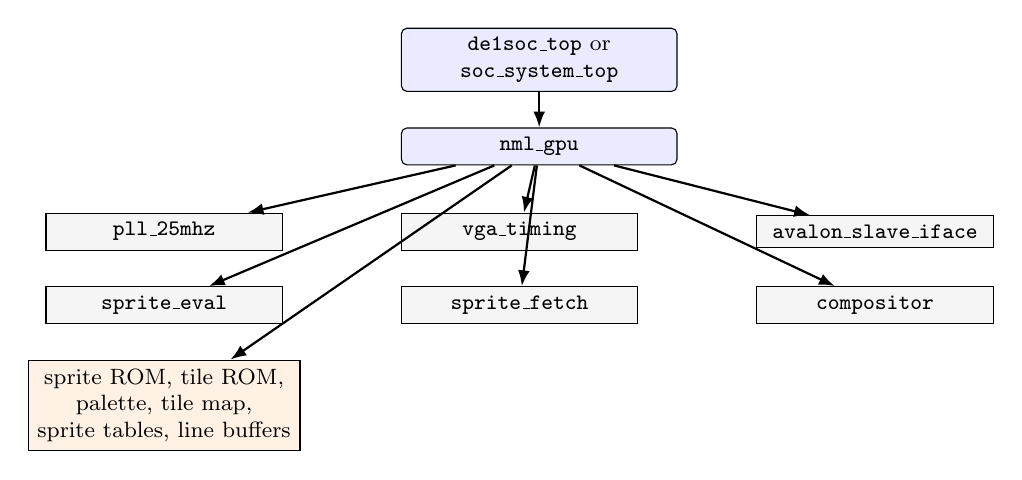
\begin{tikzpicture}[
  font=\footnotesize,
  node distance=0.45cm and 1.5cm,
  top/.style={draw, rectangle, rounded corners=2pt, fill=blue!8, minimum width=3.5cm, align=center},
  mod/.style={draw, rectangle, fill=gray!8, minimum width=3.0cm, align=center},
  mem/.style={draw, rectangle, fill=orange!10, minimum width=3.0cm, align=center},
  arr/.style={-{Latex[length=2mm]}, thick}
]
  \node[top] (top) {\texttt{de1soc\_top} or \\ \texttt{soc\_system\_top}};
  \node[top, below=of top] (gpu) {\texttt{nml\_gpu}};
  \node[mod, below left=0.6cm and 1.5cm of gpu] (pll) {\texttt{pll\_25mhz}};
  \node[mod, right=of pll] (vt) {\texttt{vga\_timing}};
  \node[mod, right=of vt] (av) {\texttt{avalon\_slave\_iface}};
  \node[mod, below=of pll] (se) {\texttt{sprite\_eval}};
  \node[mod, right=of se] (sf) {\texttt{sprite\_fetch}};
  \node[mod, right=of sf] (cp) {\texttt{compositor}};
  \node[mem, below=of se] (mem) {sprite ROM, tile ROM, \\ palette, tile map, \\ sprite tables, line buffers};

  \draw[arr] (top) -- (gpu);
  \foreach \n in {pll,vt,av,se,sf,cp} \draw[arr] (gpu) -- (\n);
  \draw[arr] (gpu) -- (mem);
\end{tikzpicture}
\caption{Module hierarchy of the GPU. The same \texttt{nml\_gpu} is wrapped by \texttt{de1soc\_top} (Phase 1) or by \texttt{soc\_system\_top} (Phase 2).}
\label{fig:hier}
\end{figure}

\subsection{Pixel clock generation (\texttt{pll\_25mhz.v})}

The VGA standard for 640$\times$480 @ 60\,Hz specifies a 25.175\,MHz pixel
clock. The Cyclone V on-chip PLL cannot produce that exact frequency from the
board's 50\,MHz reference, so we use 25\,MHz, which monitors in the lab
tolerate without issue. For the Phase 1 smoke test, the divider is a single
D flip-flop that toggles on every 50\,MHz rising edge
(\texttt{hw/pll\_25mhz.v:21--26}). Quartus promotes the divided register
output onto a global clock network when it is used as a clock downstream,
which is exactly how it is consumed in \texttt{hw/nml\_gpu.sv:194} and
elsewhere.

\begin{lstlisting}[style=sv, caption={Divide-by-2 implementation. Replace with \texttt{altera\_pll} IP in Phase 2.}]
module pll_25mhz (
    input  wire refclk,    // 50 MHz reference
    input  wire rst,       // active high reset
    output wire outclk_0   // 25 MHz pixel clock
);
    reg clk_div = 1'b0;
    always @(posedge refclk or posedge rst) begin
        if (rst) clk_div <= 1'b0;
        else     clk_div <= ~clk_div;
    end
    assign outclk_0 = clk_div;
endmodule
\end{lstlisting}

The module's port names (\texttt{refclk}, \texttt{rst}, \texttt{outclk\_0})
match the \texttt{altera\_pll} IP defaults, so the same instance signature
applies if the divider is ever replaced with the hard PLL.

The board's VGA DAC (ADV7123) samples R/G/B on its own rising edge. We drive
\texttt{vga\_clk} as the inversion of the internal pixel clock
(\texttt{hw/nml\_gpu.sv:38}) so the DAC samples in the middle of the FPGA's
hold window. This avoids hold-time violations into the DAC without adding a
register stage.

\subsection{VGA timing (\texttt{vga\_timing.sv})}

\texttt{vga\_timing} counts a horizontal axis from 0 to 799 and a vertical
axis from 0 to 524, producing standard 640$\times$480 @ 60\,Hz parameters
(\texttt{hw/vga\_timing.sv:11--21}):

\begin{table}[h]
\centering
\begin{tabular}{lrrrrr}
\toprule
Axis & Active & Front porch & Sync & Back porch & Total \\
\midrule
H    & 640    & 16          & 96   & 48         & 800   \\
V    & 480    & 10          & 2    & 33         & 525   \\
\bottomrule
\end{tabular}
\caption{VGA timing parameters for 640$\times$480 @ 60\,Hz.}
\end{table}

\texttt{hsync} and \texttt{vsync} are active low, matching the VGA spec for
this mode. \texttt{hblank} is high when \texttt{h\_count $\geq$ 640};
\texttt{vblank} is high when \texttt{v\_count $\geq$ 480};
\texttt{visible = !hblank \&\& !vblank}.

\subsection{Sprite engine}

\subsubsection{\texttt{sprite\_eval.sv}}

\texttt{sprite\_eval} is a small FSM (\texttt{IDLE $\to$ FETCH $\to$ EVAL
$\to$ DONE $\to$ IDLE}) that walks the 32-entry sprite table once per scanline
and selects the top eight sprites by priority that intersect the \emph{next}
scanline ($y + 1$). The state machine starts when the top-level asserts
\texttt{eval\_strobe} at $x = 642$, two pixels into HBLANK
(\texttt{hw/nml\_gpu.sv:248}). Each sprite is fetched in \texttt{FETCH} and
tested in \texttt{EVAL}; the test is

\begin{lstlisting}[style=sv]
intersects = spr_active &&
             (next_scanline >= spr_y) &&
             (next_scanline <  (spr_y + 16));
\end{lstlisting}

(\texttt{hw/sprite\_eval.sv:39--41}). All sprites are 16$\times$16. The
signed Y compare permits sprites to sit partly above the screen.

The insertion sort is fully unrolled (\texttt{hw/sprite\_eval.sv:77--94}):
each cycle, the incoming sprite is compared against eight registered slots; it
lands in the first empty slot or the first slot with lower priority. Slots
below the insertion point shift down by one; the lowest-priority slot is
dropped if the array is full. Total walk takes 32 cycles for fetch + eval plus
one cycle for \texttt{DONE}, well under the \textasciitilde 160-cycle HBLANK budget at
25\,MHz.

\subsubsection{\texttt{sprite\_fetch.sv}}

\texttt{sprite\_fetch} is the data-mover. Its FSM (\texttt{IDLE $\to$
CLEAR\_BUF $\to$ PROCESS\_SPRITE $\to$ READ\_PIXEL $\to$ WAIT\_PIXEL $\to$
WRITE\_PIXEL}) clears the inactive line buffer to zero (the transparent
palette index), then walks the eight sorted sprites from lowest to highest
priority, reading 16 palette-index bytes from the sprite ROM per sprite and
writing each non-zero, on-screen pixel into the line buffer
(\texttt{hw/sprite\_fetch.sv:67--131}). The \texttt{READ\_PIXEL $\to$
WAIT\_PIXEL $\to$ WRITE\_PIXEL} 3-state inner loop matches the 1-cycle read
latency of the sprite ROM (\texttt{hw/nml\_gpu.sv:194}).

A sprite is addressed by \texttt{sprrom\_raddr = (spr\_id $\ll$ 8) +
(pixel\_v $\ll$ 4) + actual\_u}, where
\texttt{actual\_u = spr\_hflip ? (15 - pixel\_u) : pixel\_u}
(\texttt{hw/sprite\_fetch.sv:107--109}). Vertical flip is in the register
layout but not wired in this revision --- only \texttt{hflip} is honoured.

Walking from lowest to highest priority is a deliberate choice: each sprite's
pixels overwrite whatever was written by a lower-priority sprite, so the
highest-priority sprite ends up on top. The buffer-clear fills with zero
(transparent) so the compositor can fall through to the tile layer where no
sprite wrote.

\subsubsection{Double line buffer}

Two 640$\times$8 line buffers (\texttt{linebuf\_A}, \texttt{linebuf\_B},
\texttt{hw/nml\_gpu.sv:198--221}) form a ping-pong pair. While
\texttt{sprite\_fetch} fills buffer A during the HBLANK after scanline $N$,
the compositor reads buffer B for scanline $N+1$; on the next HBLANK, the
selector toggles. The toggle fires when \texttt{hblank \&\& x == 640}
(\texttt{hw/nml\_gpu.sv:209}), exactly at the transition from visible to
blanking.

\subsection{Compositor (\texttt{compositor.sv})}

The compositor is a 4-stage pipeline that delivers one RGB triplet per
pixel. Figure~\ref{fig:comp} shows the stages.

\begin{figure}[h]
\centering
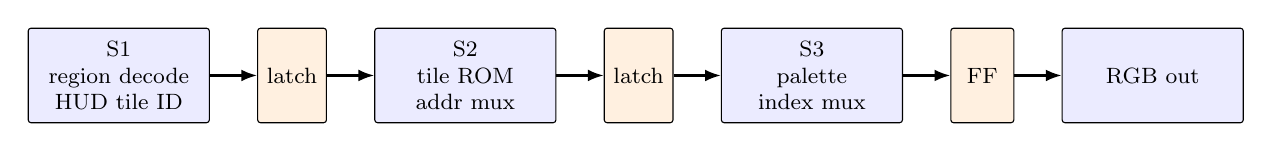
\begin{tikzpicture}[
  font=\footnotesize,
  node distance=0.4cm and 0.6cm,
  s/.style={draw, rectangle, fill=blue!8, minimum height=1.2cm, minimum width=2.3cm, align=center, rounded corners=1pt},
  l/.style={draw, rectangle, fill=orange!12, minimum height=1.2cm, minimum width=0.8cm, align=center, rounded corners=1pt},
  arr/.style={-{Latex[length=2mm]}, thick}
]
  \node[s] (s1) {S1\\region decode\\HUD tile ID};
  \node[l, right=of s1] (l1) {latch};
  \node[s, right=of l1] (s2) {S2\\tile ROM\\addr mux};
  \node[l, right=of s2] (l2) {latch};
  \node[s, right=of l2] (s3) {S3\\palette\\index mux};
  \node[l, right=of s3] (l3) {FF};
  \node[s, right=of l3] (s4) {RGB out};
  \draw[arr] (s1) -- (l1);
  \draw[arr] (l1) -- (s2);
  \draw[arr] (s2) -- (l2);
  \draw[arr] (l2) -- (s3);
  \draw[arr] (s3) -- (l3);
  \draw[arr] (l3) -- (s4);
\end{tikzpicture}
\caption{Compositor 4-stage pipeline. Tile ROM and palette RAM each contribute one register cycle.}
\label{fig:comp}
\end{figure}

The stages, with the latches between them, are
(\texttt{hw/compositor.sv:75--311}):

\begin{enumerate}[leftmargin=*]
  \item \textbf{S1 (combinational):} decode the HUD region predicates
    (\texttt{in\_hp\_bar}, \texttt{in\_ammo\_label}, \texttt{in\_ammo\_digits},
    \dots, \texttt{in\_score\_text}), compute the HUD label tile IDs from the
    local character index, and select the BCD digit nibble from
    \texttt{player\_stats}, \texttt{hud\_aux}, and \texttt{score\_reg}.
    Compute the background tile map address from $(x[9:3], y[9:3])$.
  \item \textbf{S1$\to$S2 latch} (\texttt{hw/compositor.sv:256--268}): register
    the HUD tile ID, HUD tile X/Y, HP-bar fill flag, sprite pixel from the
    line buffer, and the background tile map data.
  \item \textbf{S2 (combinational):} mux the tile ROM read address --- either
    the background path (\texttt{tile\_id, y[2:0], x[2:0]}) or the HUD glyph
    path (\texttt{hud\_tile\_id, hud\_tile\_y, hud\_tile\_x}).
  \item \textbf{S2$\to$S3 latch} (\texttt{hw/compositor.sv:280--286}): register
    the HP-bar and HUD-text flags so they line up with the tile ROM read data.
  \item \textbf{S3 (combinational):} select the palette index --- sprite pixel
    if non-zero, else the tile ROM byte (\texttt{hw/compositor.sv:289--292}).
  \item \textbf{S3$\to$S4 (registered output):} drive \texttt{rgb\_out}. HUD
    layer wins in the top 16 pixels; HP bar fills $x \in [0, 191]$ green or
    dark red; HUD glyph pixels use white on dark grey; everywhere else, the
    palette RAM output drives the line.
\end{enumerate}

Total latency from $x, y$ to \texttt{rgb\_out} is three to four cycles
(120--160\,ns at 25\,MHz), well within \texttt{VGA\_BLANK\_N} slop.

\subsection{Memories}

All six FPGA-side memories are inferred. The relevant ports and depths are
summarised in Table~\ref{tab:mem}.

\begin{table}[h]
\centering
\begin{tabular}{lllrl}
\toprule
Memory & Storage & Words$\times$Width & Bits & Used for \\
\midrule
Sprite table A & \texttt{[63:0] [0:31]} & $32\times64$ & 2{,}048 & Active sprite list \\
Sprite table B & \texttt{[63:0] [0:31]} & $32\times64$ & 2{,}048 & Shadow written by HPS \\
Palette RAM & \texttt{[23:0] [0:255]} & $256\times24$ & 6{,}144 & RGB888 colour table \\
Tile map RAM & \texttt{[3:0][7:0] [0:1199]} & $1200\times32$ & 38{,}400 & 80$\times$60 tile IDs (packed) \\
Sprite ROM & \texttt{[7:0] [0:16383]} & $16384\times8$ & 131{,}072 & 64 sprites $\times$ 256 B \\
Tile ROM & \texttt{[7:0] [0:4095]} & $4096\times8$ & 32{,}768 & 64 tiles $\times$ 64 B \\
Line buffer A & \texttt{[7:0] [0:639]} & $640\times8$ & 5{,}120 & Sprite scanline (ping) \\
Line buffer B & \texttt{[7:0] [0:639]} & $640\times8$ & 5{,}120 & Sprite scanline (pong) \\
\bottomrule
\end{tabular}
\caption{FPGA-side memory inventory.}
\label{tab:mem}
\end{table}

The sprite ROM, tile ROM, palette, and shadow sprite table are initialised
from \texttt{.hex} files via \texttt{\$readmemh} at synthesis
(\texttt{hw/nml\_gpu.sv:183--192}). The palette and sprite table are
subsequently overwritten by the HPS at runtime; the ROMs stay frozen.

Tile-map storage is unusual: the register declaration is
\texttt{logic [3:0][7:0] tilemap\_ram [0:1199]} rather than the more
obvious \texttt{logic [7:0] tilemap\_ram [0:4799]}. The reason is byte-enable
handling on the lightweight bridge. ARM emits \texttt{STRB} (single-byte
stores) for the C driver's \texttt{nml\_write\_tile()} call, and the bridge
translates them into a 32-bit write with \texttt{avs\_byteenable} selecting
one lane. With byte-organised storage, the bridge's implicit
read-modify-write would see only one byte of the word and write back zeros
for the other three, silently clobbering 75\% of the tile map
(\texttt{hw/nml\_gpu.sv:138--149}). Packed four-lane storage matches Quartus's
M10K byte-enable inference template; each \texttt{tilemap\_ram[idx][i]} lane
updates independently.

\subsection{Avalon-MM slave interface (\texttt{avalon\_slave\_iface.sv})}

The peripheral is a 32-bit lightweight Avalon-MM slave with a 14-bit
byte-address window (16\,KB). The full register map is reproduced in §5.

Reads of the scalar registers (CTRL, STATUS, BG\_SCROLL, IRQ\_MASK, player
state, HUD\_AUX) return combinationally on the read cycle. Reads of the
sprite-table, palette, and tile-map regions go through an \texttt{always\_ff}
register on \texttt{*\_rdata\_sw} lines and therefore arrive one cycle late.
To make this work without breaking the master, the slave asserts
\texttt{avs\_waitrequest} for the first cycle of any RAM-region read and
releases it on the second (\texttt{hw/avalon\_slave\_iface.sv:133--141}).

Writes to the CTRL register specifically handle \texttt{SWAP} by widening the
single-cycle Avalon strobe into a 7-cycle counter (\texttt{swap\_req\_cnt},
\texttt{hw/avalon\_slave\_iface.sv:195--209}). The widening matters because
the swap signal crosses from the 50\,MHz Avalon clock into the 25\,MHz pixel
clock, where it is captured by a three-flop synchroniser
(\texttt{hw/nml\_gpu.sv:94--106}) and edge-detected to produce a one-pulse
event in the pixel-clock domain. A single 20\,ns pulse on the Avalon side is
too narrow for the 40\,ns pixel clock to catch reliably; holding for 140\,ns
(seven 50\,MHz cycles) makes the crossing deterministic.

\subsection{Top-level integration}

\texttt{nml\_gpu.sv} is the integration shell. It instantiates the slave, the
timing generator, sprite eval, sprite fetch, the compositor, and the PLL,
and declares the inferred memories. The active and shadow sprite tables are
kept inside this file rather than inside the slave because the swap logic
lives here: when \texttt{swap\_pending} is set and \texttt{vsync} is high,
the 32-entry active table is bulk-assigned from the shadow on a single clock
edge (\texttt{hw/nml\_gpu.sv:109--118}).

\texttt{de1soc\_top.sv} is the Phase 1 wrapper. It ties the Avalon inputs off
(no master in the standalone build), wires reset to \texttt{KEY[0]}, mirrors
\texttt{VGA\_BLANK\_N} to \texttt{LEDR[1]} as a heartbeat, and passes the VGA
outputs through. The Phase 2 wrapper is \texttt{nml\_gpu\_hw/soc\_system\_top.sv},
which instantiates the Platform Designer system, exposes nml\_gpu's slave on
the HPS-to-FPGA lightweight bridge, and connects the same VGA pins.

% ===========================================================================
\section{Software Design}

The software lives in \texttt{sw/} and is structured as nine translation
units plus three headers. Three build variants share the same sources
(Table~\ref{tab:builds}).

\begin{table}[h]
\centering
\begin{tabular}{llllll}
\toprule
Variant & Target & Renderer & Input & Output \\
\midrule
\texttt{make} (default) & armhf & \texttt{render.c} & \texttt{input\_real.c} & \texttt{nml\_game} \\
\texttt{make fake-input} & armhf & \texttt{render.c} & \texttt{input\_fake.c} & \texttt{nml\_game\_fake} \\
\texttt{make terminal} & host & \texttt{render\_terminal.c} & \texttt{input\_fake.c} & \texttt{nml\_game\_term} \\
\texttt{make native} & board native & \texttt{render.c} & \texttt{input\_real.c} & \texttt{nml\_game} \\
\bottomrule
\end{tabular}
\caption{Build variants (\texttt{sw/Makefile:42--72}).}
\label{tab:builds}
\end{table}

The terminal build also defines \texttt{NML\_TERMINAL\_BUILD}, which compiles
out the FPGA paths in \texttt{main.c}.

\subsection{Game state machine and entity pool (\texttt{game.c}, \texttt{game.h})}

State is held in a single struct (\texttt{sw/game.h:93--133}). The active
states are \texttt{STATE\_PLAYING}, \texttt{STATE\_LEVELUP}, and
\texttt{STATE\_GAMEOVER}. A fixed-size pool of 64 entities
(\texttt{MAX\_ENTITIES}, \texttt{sw/game.h:6}) holds the player, enemies,
bullets, hazards, and ammo drops. Each entity tracks kind, active flag,
position, velocity, hp, an animation phase, a TTL, a payload, and a fire
cooldown (\texttt{sw/game.h:79--90}).

\texttt{game\_tick()} (\texttt{sw/game.c:428--485}) dispatches on state:

\begin{itemize}[leftmargin=*,nosep]
  \item In \texttt{STATE\_PLAYING}, it updates the player, runs the wave
    spawner, moves enemies, advances bullets, ages hazards, runs auto-attack
    timers, and resolves collisions. On wave clear it transitions to
    \texttt{STATE\_LEVELUP}. On HP $\leq 0$ it transitions to
    \texttt{STATE\_GAMEOVER} and deactivates every entity including the
    player so the death screen has a clean tilemap to draw into.
  \item In \texttt{STATE\_LEVELUP}, the player picks one of three offered
    weapons with the D-pad and confirms with the B button
    (\texttt{sw/game.c:416--426}). On confirm, the chosen weapon is upgraded
    and the next wave starts.
  \item In \texttt{STATE\_GAMEOVER}, START restarts the game by re-calling
    \texttt{game\_init()}.
\end{itemize}

Enemy motion (\texttt{sw/game.c:219--254}) is a per-enemy random walk in X
combined with vertical pursuit of the player. The walk decision re-rolls
every 12 frames (\texttt{ENEMY\_DIR\_FRAMES}) using a per-enemy seed
(\texttt{phase}) so the cohort does not collapse into a single column where
the player's bullet stream would mop them up trivially. Armed enemies also
fire bullets back on a per-enemy cooldown jittered at spawn
(\texttt{sw/game.c:21--23, 239--246}).

Collision resolution is AABB at 16$\times$16 (\texttt{sw/game.c:298--312}).
All kills go through \texttt{apply\_damage()} (\texttt{sw/game.c:318--333})
so that score, kill counter, and ammo-drop probability are recorded uniformly
across weapon paths. The drop probability is 30\% per kill
(\texttt{sw/game.h:144}, \texttt{AMMO\_DROP\_PERCENT}).

\subsection{Wave system (\texttt{wave.c}, \texttt{wave.h})}

The wave table is a hard-coded array of five entries (\texttt{sw/wave.c:9--16}):

\begin{table}[h]
\centering
\begin{tabular}{rrrrrr}
\toprule
Wave & Spawn period (frames) & Total & Armed & Armed HP & Speed \\
\midrule
1 & 60 & 6 & 0 & 1 & 1 \\
2 & 50 & 8 & 1 & 2 & 1 \\
3 & 45 & 10 & 2 & 2 & 2 \\
4 & 35 & 12 & 4 & 2 & 2 \\
5 & 25 & 16 & 6 & 3 & 3 \\
\bottomrule
\end{tabular}
\end{table}

After wave 5 the table clamps to its last entry, so the game can keep running
indefinitely at maximum difficulty. \texttt{wave\_advance()} top-ups ammo
(+40, capped at 99), artillery (+2, capped at 5), and gas (+2, capped at 5)
on every transition out of \texttt{STATE\_LEVELUP}.

\subsection{Auto-attack system (\texttt{autoatk.c}, \texttt{autoatk.h})}

Three auto-attack kinds exist (\texttt{sw/game.h:60--65}):

\begin{itemize}[leftmargin=*]
  \item \textbf{Mortar} is timer-driven. At level 1 it fires every 180 frames,
    decreasing by 30 frames per upgrade, floored at 60 frames
    (\texttt{sw/autoatk.c:10--20, 39--45}). Each shell launches upward from
    the player's column with random horizontal jitter and a TTL of 200 frames.
  \item \textbf{Artillery} is player-triggered with the L shoulder button. On
    fire it kills every enemy in a 16-pixel column above the player
    (\texttt{sw/autoatk.c:200--219}) and paints a vertical column of
    \texttt{TILE\_BEAM} glyphs into the tile map for six frames as the visual
    effect.
  \item \textbf{Mustard gas} is player-triggered with the R shoulder. It
    spawns a single \texttt{ENT\_HAZARD} at the player's position with a TTL
    of 90 frames. The cloud grows from 16$\times$16 px to 48$\times$32 px
    over the first 30 frames, holds, and shrinks over the last 15
    (\texttt{sw/autoatk.c:160--178}).
\end{itemize}

Each weapon has a per-button input cooldown of 20 frames
(\texttt{ABILITY\_INPUT\_COOLDOWN}, \texttt{sw/game.h:145}) to debounce noisy
SNES shoulder buttons.

\subsection{Input subsystem}

The input API is a single function:
\texttt{uint16\_t input\_read(int frame)} (\texttt{sw/input.h:6}). Either
\texttt{input\_real.c} (the DragonRise reader) or \texttt{input\_fake.c}
(the deterministic stub) is linked.

The real reader opens \texttt{/dev/input/event0} (the only evdev node that
shows up for the gamepad on the DE1-SoC kernel --- \texttt{joydev} is not
built in, so there is no \texttt{/dev/input/js0}). It drains pending events
on every call, updating an internal button bitmask and axis values
(\texttt{sw/input\_real.c:127--147}). The D-pad is reported as
\texttt{ABS\_X}/\texttt{ABS\_Y}; axes are converted to four directional bits
with a deadzone equal to a quarter of the reported range, queried via
\texttt{EVIOCGABS} so the same code works whether the pad reports $-1..1$,
$0..255$, or signed 16-bit values.

\subsection{Rendering pipeline (\texttt{render.c}, \texttt{render\_terminal.c})}

\texttt{render\_frame()} (\texttt{sw/render.c:342--421}) is called once per
tick. It writes the entity pool into the FPGA sprite table:

\begin{itemize}[leftmargin=*,nosep]
  \item Slot 0 is always the player.
  \item Slots 1--31 hold active non-player entities in pool order.
  \item Gas hazards expand into up to four sprite slots
    (\texttt{sw/render.c:98--111}).
  \item Bullets get priority 2 (low), enemies and hazards priority 1, the
    player priority 0 (high).
\end{itemize}

Leftover slots are explicitly hidden by \texttt{nml\_hide\_sprite()} so prior
frames do not ghost (\texttt{sw/render.c:407--409}). The HUD mailbox
registers are updated every frame.

The terminal renderer (\texttt{sw/render\_terminal.c}) mirrors the slot
allocation logic exactly but prints each sprite slot to stdout as an ASCII
glyph. This lets the game logic be exercised in CI and on a laptop without
hardware.

\subsection{Main loop (\texttt{main.c})}

\texttt{main()} (\texttt{sw/main.c:171--274}) is a fixed-timestep 60\,Hz loop:

\begin{enumerate}[leftmargin=*,nosep]
  \item Read input (\texttt{input\_read}).
  \item Tick the game (\texttt{game\_tick}).
  \item Render (\texttt{render\_frame} writes the sprite table).
  \item Commit (\texttt{nml\_commit\_frame()} sets \texttt{CTRL.SWAP}, then
    polls \texttt{STATUS.SWAP\_PENDING} until it clears or a 200{,}000-iteration
    timeout trips).
  \item Sleep the remainder of the 16{,}666\,$\mu$s frame budget.
\end{enumerate}

On the host (terminal build), \texttt{nml\_commit\_frame()} is
\texttt{\#ifdef}-ed out and \texttt{nanosleep} is the sole pacing source. On
the board, the SWAP poll synchronises the loop with VBLANK.

Palette initialisation happens once at startup
(\texttt{init\_palette\_runtime()}, \texttt{sw/main.c:139--168}). The HPS
writes sixteen entries covering player, enemies, projectiles, dirt, grass,
and the white sprite border. This step shadows the \texttt{\$readmemh}
initialisation; once it runs, the software is the authoritative source of
palette data.

% ===========================================================================
\section{Hardware--Software Interface}

The peripheral occupies 16\,KB starting at \texttt{0xFF200000} in HPS
physical address space (the lightweight bridge base on the DE1-SoC). The
userspace driver \texttt{mmap()}s the whole window via \texttt{/dev/mem}
(\texttt{sw/nml\_gpu.c:33--59}) and exposes typed writers.

\subsection{Register map}

\begin{longtable}{lp{2.7cm}rcp{6.6cm}}
\toprule
Offset & Name & W & Acc. & Layout \\
\midrule
\endhead
\texttt{0x0000} & \texttt{CTRL} & 32 & R/W & \texttt{[0]=ENABLE}, \texttt{[1]=SWAP} (auto-clear), \texttt{[2]=HUD\_ON} \\
\texttt{0x0004} & \texttt{STATUS} & 32 & R & \texttt{[0]=VBLANK}, \texttt{[1]=SWAP\_PENDING}, \texttt{[15:8]=frame\_ctr} (wired 0 at present) \\
\texttt{0x0008} & \texttt{BG\_SCROLL} & 32 & R/W & \texttt{[15:0]=scroll\_x} (signed), \texttt{[31:16]=scroll\_y} (signed) \\
\texttt{0x000C} & \texttt{IRQ\_MASK} & 32 & R/W & \texttt{[0]=VBLANK IRQ enable} (Phase 2; wired 0 here) \\
\texttt{0x0010} & \texttt{PLAYER\_POS} & 32 & R/W & \texttt{[15:0]=px}, \texttt{[31:16]=py} \\
\texttt{0x0014} & \texttt{PLAYER\_STATS} & 32 & R/W & \texttt{[7:0]=hp}, \texttt{[15:8]=wave} BCD (2 digits), \texttt{[31:16]=level} \\
\texttt{0x0018} & \texttt{SCORE} & 32 & R/W & \texttt{[23:0]=score} BCD (6 digits) \\
\texttt{0x001C} & \texttt{KILL\_COUNT} & 32 & R/W & 32-bit kill counter (HUD-only, optional) \\
\texttt{0x0020} & \texttt{HUD\_AUX} & 32 & R/W & \texttt{[7:0]=ammo} BCD (2 digits), \texttt{[11:8]=art}, \texttt{[15:12]=gas} \\
\texttt{0x0100--0x01FF} & Sprite table & 256\,B & R/W & 32 $\times$ 8\,B entries \\
\texttt{0x0400--0x07FF} & Palette & 1\,KB & R/W & 256 $\times$ 4\,B; \texttt{[23:0]=RGB888} \\
\texttt{0x1000--0x22BF} & Tile map & 4.7\,KB & R/W & 80$\times$60 bytes; byte = tile ID \\
\bottomrule
\caption{Avalon-MM register map.}\label{tab:regmap}
\end{longtable}

Each sprite-table entry is two 32-bit words:

\begin{table}[h]
\centering
\begin{tabular}{lll}
\toprule
Word & Bits & Field \\
\midrule
W0 & 15:0 & \texttt{x} (signed) \\
W0 & 31:16 & \texttt{y} (signed) \\
W1 & 7:0 & \texttt{sprite\_id} \\
W1 & 15:8 & \texttt{flags} \\
W1 & 23:16 & \texttt{palette\_off} \\
W1 & 31:24 & reserved \\
\bottomrule
\end{tabular}
\end{table}

The \texttt{flags} byte packs (\texttt{sw/nml\_gpu.h:58--69}): bit 2 hflip,
bit 3 vflip, bits 6:4 priority (0 = highest), bit 7 ACTIVE. The
\texttt{ACTIVE} bit is the flag that \texttt{sprite\_eval} actually checks at
bit 47 of the 64-bit packed word; the original design used sentinel
coordinates exclusively, but the hardware now also honours the explicit
active bit (\texttt{sw/nml\_gpu.h:12--16}, \texttt{hw/sprite\_eval.sv:32--34}).

\subsection{Frame-commit handshake}

The frame-commit sequence is:

\begin{enumerate}[leftmargin=*,nosep]
  \item CPU writes the sprite table, palette, tile map, player state, and
    HUD aux fields. All writes land in shadow registers/RAMs immediately.
  \item CPU writes \texttt{CTRL.SWAP = 1}. The slave widens the strobe to
    seven 50\,MHz cycles (\texttt{hw/avalon\_slave\_iface.sv:199--209}),
    so the pixel clock can synchronise the request through three flip-flops
    and capture an edge (\texttt{hw/nml\_gpu.sv:94--106}). \texttt{SWAP}
    auto-clears in the same cycle it was written.
  \item At the next VSYNC, the 32-entry sprite table is bulk-assigned from
    shadow to active in one clock edge (\texttt{hw/nml\_gpu.sv:113--118}).
    \texttt{swap\_pending} clears.
  \item CPU polls \texttt{STATUS.SWAP\_PENDING} until it falls or the
    200{,}000-iteration timeout trips (\texttt{sw/nml\_gpu.c:179--190}).
\end{enumerate}

The palette and tile map do not go through the swap handshake. Both have one
logical bank that is written in the Avalon clock domain and read in the pixel
clock domain. Visible artefacts from mid-frame writes are possible in theory;
in practice palette and tile updates are rare, so we left it that way.

\subsection{Byte-store semantics for the tile map}

\texttt{nml\_write\_tile()} issues a single-byte \texttt{STRB} to the tile-map
region (\texttt{sw/nml\_gpu.c:92--99}). The lightweight bridge translates this
into a 32-bit Avalon write with \texttt{avs\_byteenable} set to one nibble.
On the slave side, the packed-byte tile-map storage \texttt{logic [3:0][7:0]
tilemap\_ram} exposes four byte-enable lanes per M10K word and writes only
the addressed lane (\texttt{hw/nml\_gpu.sv:158--162}). Reads return the full
word; the pixel side selects one of the four bytes per pixel based on
\texttt{tilemap\_raddr[1:0]} (\texttt{hw/nml\_gpu.sv:169--173}).

This packed layout is non-obvious but is the difference between a correct
tile map and one where only every fourth column receives the write.

% ===========================================================================
\section{Build and Toolchain}

\subsection{Hardware build}

Quartus Prime Lite 21.1 is the synthesis and place-and-route tool. Two flows
exist.

\textbf{Phase 1 (\texttt{hw/quartus/}).} A standalone bitstream that places
\texttt{nml\_gpu} inside \texttt{de1soc\_top} with the Avalon slave tied off.
The four \texttt{.hex} files generated by \texttt{hw/gen\_rom.py} are picked
up via \texttt{\$readmemh} at synthesis time, courtesy of
\texttt{SEARCH\_PATH ".."} in the QSF (\texttt{hw/quartus/nml\_gpu.qsf}).
Compilation runs in 63\,s on a lab machine and produces
\texttt{output\_files/nml\_gpu.sof} (for JTAG) and
\texttt{output\_files/nml\_gpu.rbf} (raw binary for SD-card boot).

\textbf{Phase 2 (\texttt{nml\_gpu\_hw/}).} A Platform Designer system with an
HPS instance, a clock bridge, an AXI-to-Avalon adapter on the HPS-to-FPGA
lightweight bridge, and the nml\_gpu component as an Avalon slave. The
component descriptor lives in \texttt{nml\_gpu\_hw.tcl} and sets the
device-tree metadata (\texttt{compatible = "csee4840,nml\_gpu-1.0"}) so the
kernel exposes the peripheral at
\texttt{/proc/device-tree/sopc@0/bridge@0xc0000000/vga@0x100000000/}.

\subsection{ROM generation (\texttt{hw/gen\_rom.py})}

\texttt{gen\_rom.py} is a 777-line Python script that emits four hex files:
\texttt{sprite\_rom.hex} (16\,384 bytes), \texttt{tile\_rom.hex} (4\,096
bytes), \texttt{palette.hex} (256 RGB888 entries), and
\texttt{sprite\_table.hex} (32 initial sprite slots).

\subsection{Software build}

The userspace binary cross-compiles with \texttt{arm-linux-gnueabihf-gcc}
(\texttt{sw/Makefile:23}). It links statically (\texttt{-static}) so it runs
on the board without a matching glibc, and uses standard POSIX APIs
(\texttt{/dev/mem}, \texttt{mmap}, evdev, \texttt{nanosleep},
\texttt{clock\_gettime}). No threading; everything is in one process loop.

\subsection{Boot and SD-card image}

The Phase 2 image follows the standard DE1-SoC Linux boot flow: preloader
$\to$ U-Boot $\to$ kernel (Linux 4.19 from \texttt{altera-fpga/linux-socfpga})
$\to$ root filesystem on the ext4 partition. The FPGA RBF and DTB sit on the
FAT boot partition. U-Boot loads the bitstream into the FPGA fabric before
launching the kernel, so the smoke-test scene is already on the VGA monitor
by the time userspace comes up. After login, the operator copies
\texttt{nml\_game} onto the board and runs it as root.

% ===========================================================================
\section{Testing and Verification}

Three test rungs:

\begin{itemize}[leftmargin=*]
  \item \textbf{Phase 0 (host).} \texttt{cd sw \&\& make terminal \&\&
    ./nml\_game\_term} runs the entire game loop without hardware, printing
    every frame's sprite table to stdout. The deterministic input stub
    exercises every weapon path on a fixed cycle.
  \item \textbf{Phase 1 (FPGA only).} With the \texttt{.sof} loaded over JTAG,
    the monitor shows the smoke-test scene (dark battlefield, green player
    square, two red enemies, a yellow bullet) within one second. This proves
    the entire pixel pipeline.
  \item \textbf{Phase 2 (HPS-integrated).} With the RBF and DTB on the SD
    card, the kernel exposes the peripheral, and \texttt{./nml\_game} mmaps
    it. The game loop runs at 60\,Hz, the controller drives the player, the
    VGA monitor displays the rendered frame, and the terminal logs wave
    starts and clears.
\end{itemize}

% ===========================================================================
\section{Results}

\subsection{Resource utilisation}

From \texttt{hw/quartus/output\_files/nml\_gpu.fit.summary} (Phase 1 build,
Cyclone V SE 5CSEMA5F31C6):

\begin{table}[h]
\centering
\begin{tabular}{lrrr}
\toprule
Resource & Used & Available & Fraction \\
\midrule
ALMs & 205 & 32{,}070 & $<\,1\%$ \\
Registers & 365 & --- & --- \\
Pins & 54 & 457 & 12\% \\
Block memory bits & 86{,}144 & 4{,}065{,}280 & 2\% \\
M10K blocks & 14 & 397 & 4\% \\
DSP blocks & 0 & 87 & 0\% \\
PLLs & 0 & 6 & 0\% \\
\bottomrule
\end{tabular}
\caption{Phase 1 resource utilisation.}
\end{table}

Total compile time: 63\,s (Analysis \& Synthesis 13\,s, Fitter 30\,s,
Assembler 12\,s, Timing Analyzer 8\,s).

\subsection{Timing analysis}

\texttt{hw/quartus/output\_files/nml\_gpu.sta.summary} reports negative slack
on the slow-1100mV-85$^\circ$C corner:

\begin{table}[h]
\centering
\begin{tabular}{llrr}
\toprule
Corner & Clock & Setup slack & TNS \\
\midrule
Slow 1100mV 85$^\circ$C & \texttt{clk\_div} & $-5.111$\,ns & $-1409.97$\,ns \\
Slow 1100mV 85$^\circ$C & \texttt{CLOCK\_50} & $-3.506$\,ns & $-3.506$\,ns \\
Fast 1100mV 85$^\circ$C & \texttt{clk\_div} & $-2.654$\,ns & $-725.39$\,ns \\
\bottomrule
\end{tabular}
\end{table}

All hold checks pass. The dominant violation is a minimum-pulse-width report
on the divided clock register. The pixel-clock domain runs at 25\,MHz
(40\,ns period), but the timing analyser treats the divider register as if
it were producing a much higher-frequency clock; the combination of
\texttt{posedge} and \texttt{negedge} from the alternating toggle makes the
analyser see a 20\,ns half-period. On real silicon the register is promoted
to the global clock network and the duty cycle is exact, so the divider
works as intended --- but the analyser cannot see that, and reports failure.

The cleaner alternative is to drive the pixel clock from an
\texttt{altera\_pll} IP instance configured for 25\,MHz, which the analyser
models correctly. The Phase 1 board passes timing visually at lab temperature
on the divider, and the divider's port signature matches the IP defaults, so
the swap remains a drop-in if the analyser numbers ever need to be clean.

\subsection{Frame timing}

In the deployed (Phase 2) configuration, \texttt{top -n 1 -b} while
\texttt{nml\_game} is running shows CPU usage under 5\%. The loop spends most
of its time in \texttt{nanosleep} or polling \texttt{STATUS.SWAP\_PENDING}
inside \texttt{nml\_commit\_frame()}.

% ===========================================================================
\section{Challenges and Resolutions}

\subsection{Tile-map byte-enable RMW}

The original tile-map storage was \texttt{logic [7:0] tilemap\_ram [0:4799]}
--- one byte per word. The Linux driver's \texttt{nml\_write\_tile()} issues
an ARM \texttt{STRB} for each tile update. The HPS-to-FPGA lightweight bridge
sets \texttt{avs\_byteenable} to one nibble and the Avalon slave's effective
behaviour was a read-modify-write: read the 32-bit word, mask in the new
byte, write back. With byte-organised storage, the slave only returned one
byte from each read, so the bridge masked three zero bytes into the other
lanes and silently clobbered them. The visible symptom was that only every
fourth tile column showed new content; the rest stayed at reset value 0.

The fix is the packed \texttt{logic [3:0][7:0] tilemap\_ram [0:1199]}
storage plus a per-lane write in \texttt{hw/nml\_gpu.sv:158--162}. Each lane
updates independently, and reads return all four bytes, so the bridge's
read-modify-write preserves the untouched bytes.

\subsection{Single-cycle \texttt{eval\_done} against multi-cycle \texttt{CLEAR\_BUF}}

\texttt{sprite\_eval} finishes its 32-sprite walk in roughly 33 cycles and
asserts \texttt{eval\_done} for one cycle. \texttt{sprite\_fetch} is in
\texttt{CLEAR\_BUF} for 640 cycles (one write per pixel) and only checks
\texttt{eval\_done} once, at the end of the buffer clear. If the eval pulse
fires while fetch is still mid-clear, the pulse is gone by the time fetch
samples it.

The first fix attempted was to edge-detect a transition on
\texttt{active\_mask}. That worked for the smoke-test scene because the
active set changes between non-sprite and sprite rows. It silently failed
for the game's much busier scenes: 15 of every 16 scanlines inside a
16-pixel sprite see the \emph{same} active set, so no transition fires.

The current fix is a sustain latch: \texttt{eval\_done\_r} is set when the
pulse arrives and cleared at the next \texttt{eval\_strobe}.
\texttt{sprite\_fetch} samples \texttt{eval\_done\_r} and is guaranteed to
see it set after the first eval of a line, regardless of when fetch happens
to check (\texttt{hw/nml\_gpu.sv:264--270}).

\subsection{CDC on \texttt{ctrl\_swap\_req}}

\texttt{CTRL.SWAP} is written from the 50\,MHz Avalon clock and consumed in
the 25\,MHz pixel clock. The straight single-cycle pulse from the slave was
20\,ns wide; a two-flop synchroniser at 25\,MHz samples every 40\,ns, so it
could easily miss the pulse entirely.

The slave now widens the request: a 3-bit counter loaded with 7 on each
SWAP write holds \texttt{ctrl\_swap\_req} high for seven 50\,MHz cycles
(140\,ns), which is enough that a three-flop chain on the pixel side
captures the rising edge deterministically.

\subsection{Pixel-clock duty cycle}

The divide-by-2 register works on silicon but fails the analyser's
minimum-pulse-width check. We documented the failure mode; the divider's
port names match the \texttt{altera\_pll} IP defaults, so any later
replacement is a drop-in.

% ===========================================================================
\section{Conclusion}

The Phase 1 smoke-test bitstream works as designed on hardware: 640$\times$480
@ 60\,Hz, tile + sprite + palette + HUD pipeline, full VGA pin set. The
Phase 2 HPS-integrated build boots Linux, exposes the peripheral on the
lightweight bridge, runs the C game at 60\,Hz, and reads SNES controller
input via evdev. Player movement, firing, enemy spawning, wave progression,
level-up, mortar timers, artillery, gas clouds, ammo drops, and the HUD
numerics all function in the deployed configuration.

The project demonstrates a complete hardware/software co-design: a custom
SystemVerilog GPU peripheral in the Cyclone V fabric handles rendering, while
the ARM Cortex-A9 runs the game logic and writes sprite tables, palette, and
player state through a 16\,KB Avalon-MM slave with a tear-free VBLANK swap.
The partition keeps the CPU free of pixel work and gives the design headroom
for richer gameplay within the same memory and bandwidth budget.

% ===========================================================================
\section*{References}
\addcontentsline{toc}{section}{References}

\begin{enumerate}[leftmargin=*,nosep]
  \item \texttt{DESIGN.md} --- Project design document, April 2026.
  \item \texttt{SETUP.md} --- Bring-up instructions for Phase 0, Phase 1, and Phase 2.
  \item Terasic Inc., \emph{DE1-SoC User Manual}, Revision 1.2.4.
  \item Intel/Altera, \emph{Cyclone V Device Handbook} (Volume 1).
  \item Intel/Altera, \emph{Avalon Interface Specifications}, MNL-AVABUSREF.
  \item Analog Devices, \emph{ADV7123 Triple High-Speed Video DAC Datasheet}.
  \item VESA, \emph{VGA 640$\times$480 @ 60\,Hz timing specification}.
  \item Linux kernel evdev documentation: \texttt{Documentation/input/event-codes.rst}.
  \item \texttt{lab3-reference/CSEE4840W-Lab3} --- VGA ball lab providing the timing-generator skeleton.
\end{enumerate}

% ===========================================================================
\appendix
\section*{Appendix: Source Listings}
\addcontentsline{toc}{section}{Appendix: Source Listings}

This appendix reproduces the complete source for the hardware and software
components of the project, as built and run on the DE1-SoC.

\subsection*{Hardware (\texttt{hw/})}

\subsection*{\texttt{de1soc\_top.sv}}
\lstinputlisting[style=sv]{../hw/de1soc_top.sv}

\subsection*{\texttt{nml\_gpu.sv}}
\lstinputlisting[style=sv]{../hw/nml_gpu.sv}

\subsection*{\texttt{avalon\_slave\_iface.sv}}
\lstinputlisting[style=sv]{../hw/avalon_slave_iface.sv}

\subsection*{\texttt{vga\_timing.sv}}
\lstinputlisting[style=sv]{../hw/vga_timing.sv}

\subsection*{\texttt{sprite\_eval.sv}}
\lstinputlisting[style=sv]{../hw/sprite_eval.sv}

\subsection*{\texttt{sprite\_fetch.sv}}
\lstinputlisting[style=sv]{../hw/sprite_fetch.sv}

\subsection*{\texttt{compositor.sv}}
\lstinputlisting[style=sv]{../hw/compositor.sv}

\subsection*{\texttt{pll\_25mhz.v}}
\lstinputlisting[style=sv]{../hw/pll_25mhz.v}

\subsection*{\texttt{gen\_rom.py}}
\lstinputlisting[style=plain]{../hw/gen_rom.py}

\subsection*{Software (\texttt{sw/})}

\subsection*{\texttt{main.c}}
\lstinputlisting[style=c]{../sw/main.c}

\subsection*{\texttt{game.h}}
\lstinputlisting[style=c]{../sw/game.h}

\subsection*{\texttt{game.c}}
\lstinputlisting[style=c]{../sw/game.c}

\subsection*{\texttt{wave.h}}
\lstinputlisting[style=c]{../sw/wave.h}

\subsection*{\texttt{wave.c}}
\lstinputlisting[style=c]{../sw/wave.c}

\subsection*{\texttt{autoatk.h}}
\lstinputlisting[style=c]{../sw/autoatk.h}

\subsection*{\texttt{autoatk.c}}
\lstinputlisting[style=c]{../sw/autoatk.c}

\subsection*{\texttt{input.h}}
\lstinputlisting[style=c]{../sw/input.h}

\subsection*{\texttt{input\_real.c}}
\lstinputlisting[style=c]{../sw/input_real.c}

\subsection*{\texttt{input\_fake.c}}
\lstinputlisting[style=c]{../sw/input_fake.c}

\subsection*{\texttt{render.h}}
\lstinputlisting[style=c]{../sw/render.h}

\subsection*{\texttt{render.c}}
\lstinputlisting[style=c]{../sw/render.c}

\subsection*{\texttt{render\_terminal.c}}
\lstinputlisting[style=c]{../sw/render_terminal.c}

\subsection*{\texttt{nml\_gpu.h}}
\lstinputlisting[style=c]{../sw/nml_gpu.h}

\subsection*{\texttt{nml\_gpu.c}}
\lstinputlisting[style=c]{../sw/nml_gpu.c}

\subsection*{\texttt{Makefile}}
\lstinputlisting[style=plain]{../sw/Makefile}

\end{document}
